%---------------------------------------------------------------------
\section{Resultados das simula��es}

Nas simula��es, procuramos avaliar o comportamento do sistema para as seguintes condi��es:
%
\begin{enumerate*}[label=(\roman*)]
\item condi��o inicial $y(0)$;
\item par�metros da planta;
\item sinal de refer�ncia;
\item ganho de adapta��o $\Gamma$.
\end{enumerate*}

Apresentaremos os resultados obtidos atrav�s de simula��es no ambiente \HI{\texttt{Matlab/Simulink}} e os discutiremos na pr�xima se��o.
%
Para todas as simula��es, utilizamos $k^\intercal = \mat{1 & 1}$, $c_1 = c_2 = d_1 = d_2 = \gamma = 1$ e condi��es iniciais nulas em todas as din�micas, exceto em $\rho(0) = 1$ e $y(0)$.

\subsection{Simula��o \#1}

Inicialmente, desejamos verificar o comportamento do sistema para varia��es nas
condi��es iniciais.

%
\begin{align*}
  y &= \frac{5}{s^2+2s+1}u\,,  &  y(0) &= \HI{0} \, \textrm{e} \, \HI{10}\,,
  & \Gamma &= 1 \, \textbf{I}_3\,, & y_r &= \textrm{sin}(t) +
  \textrm{sin}(3t) \, .
\end{align*}
%
\begin{figure}[H]
  \centering
  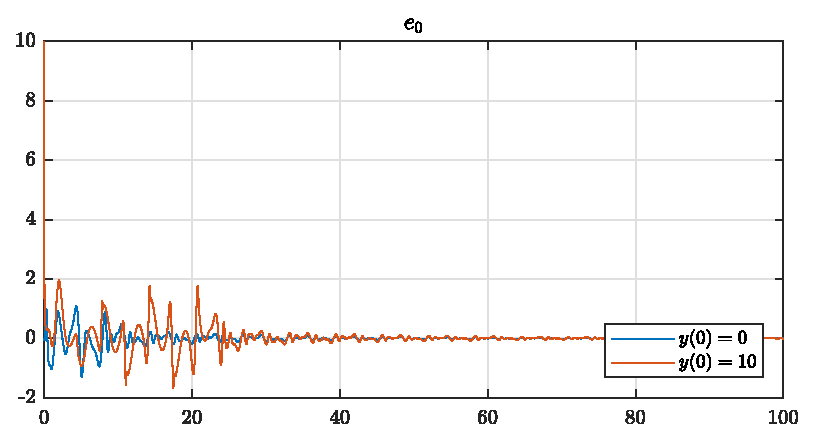
\includegraphics[width=12cm]{figs/e0/y01y02.eps} 
\end{figure}

\begin{figure}[H]
  \centering
  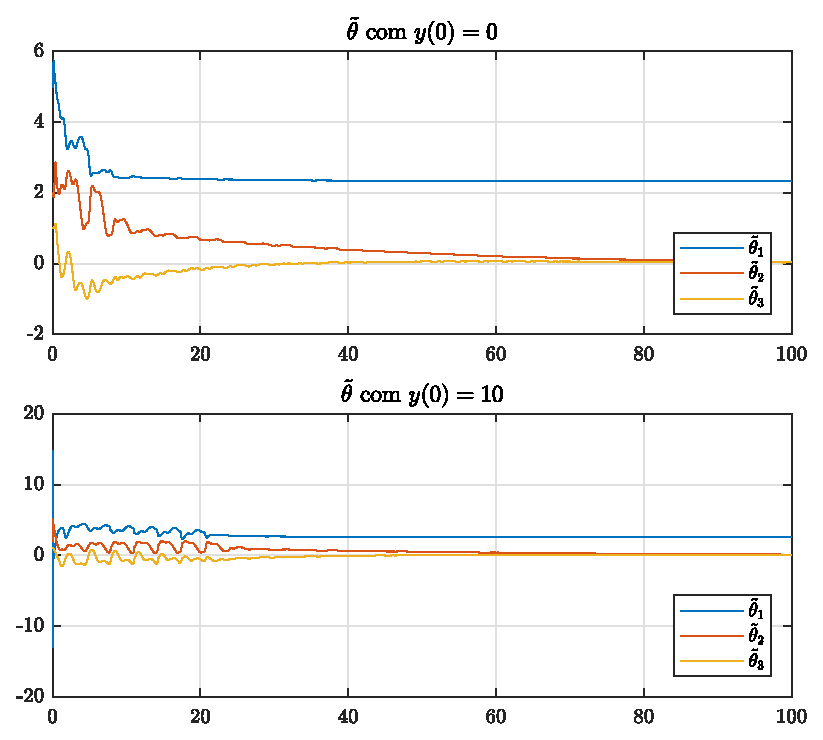
\includegraphics[width=12cm]{figs/tiltheta/y01y02.eps} 
\end{figure}

\begin{figure}[H]
  \centering
  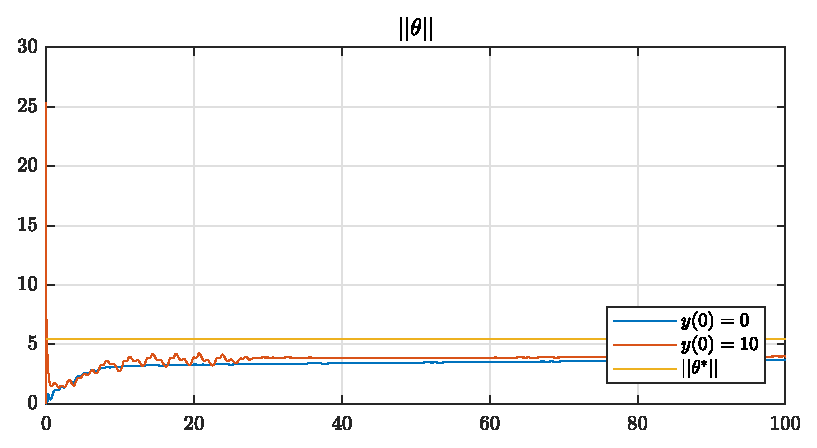
\includegraphics[width=12cm]{figs/modtheta/y01y02.eps} 
\end{figure}

\begin{figure}[H]
  \centering
  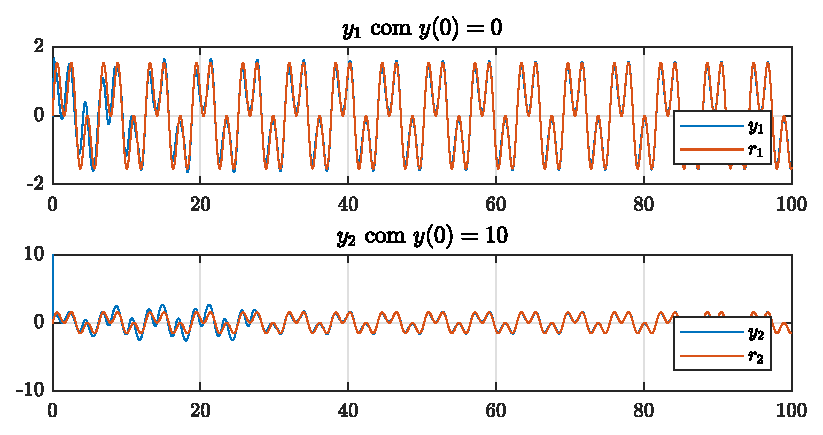
\includegraphics[width=12cm]{figs/y/y01y02.eps} 
\end{figure}

\begin{figure}[H]
  \centering
  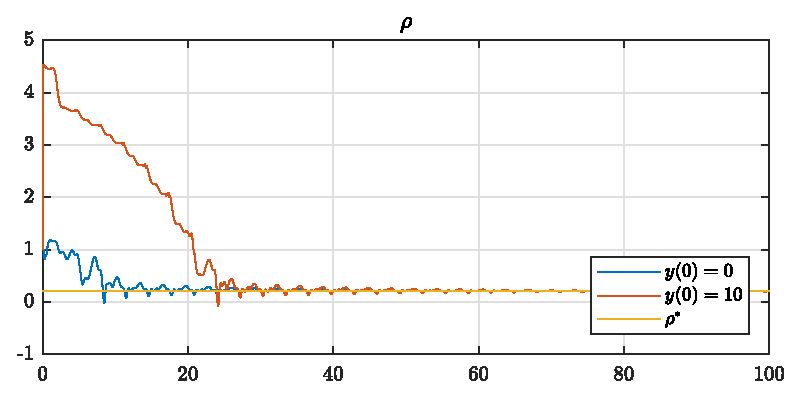
\includegraphics[width=12cm]{figs/rho/y01y02.eps} 
\end{figure}

\subsection{Simula��o \#2}

Verificamos o comportamento do sistema para varia��es nos par�metros da planta.

\begin{align*}
  y &= \HI{$\frac{5}{s^2+2s+1}u$} \,\,\, \textrm{e} \,\,\, \HI{$\frac{2}{s^2-2s+1}u$} \,,  &   y(0) &=  0 \,, & \Gamma &= 1 \,
  \textbf{I}_3\,, & y_r &= \textrm{sin}(t) + \textrm{sin}(3t) \, .
\end{align*}

\begin{figure}[H]
  \centering
  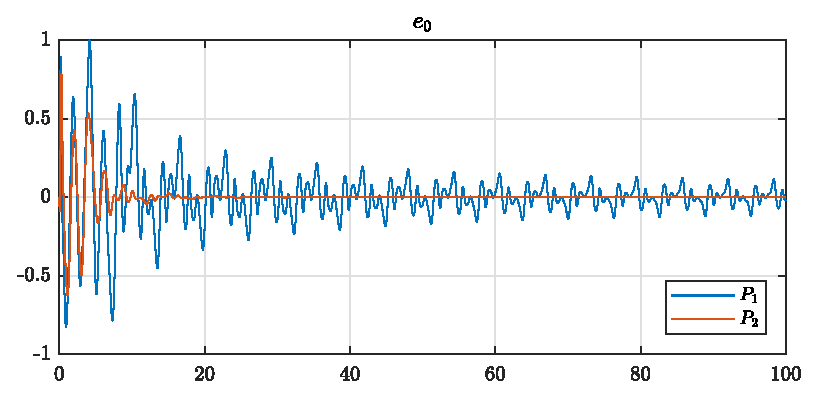
\includegraphics[width=12cm]{figs/e0/P1P2.eps} 
\end{figure}

\begin{figure}[H]
  \centering
  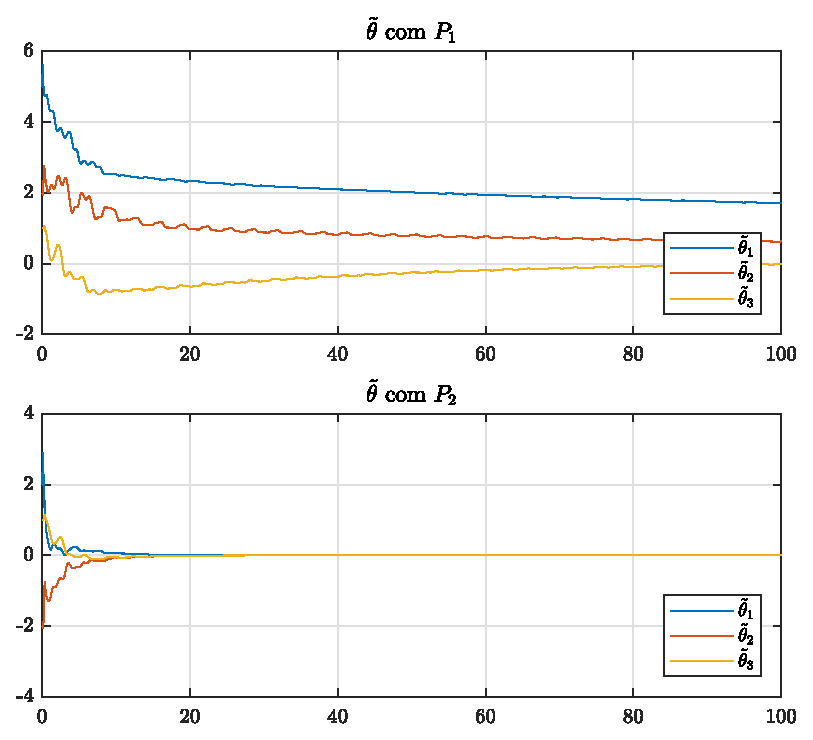
\includegraphics[width=12cm]{figs/tiltheta/P1P2.eps} 
\end{figure}

\begin{figure}[H]
  \centering
  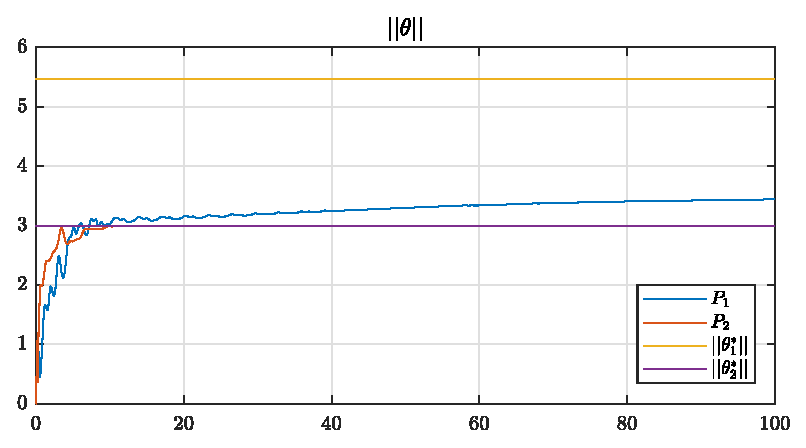
\includegraphics[width=12cm]{figs/modtheta/P1P2.eps} 
\end{figure}

\begin{figure}[H]
  \centering
  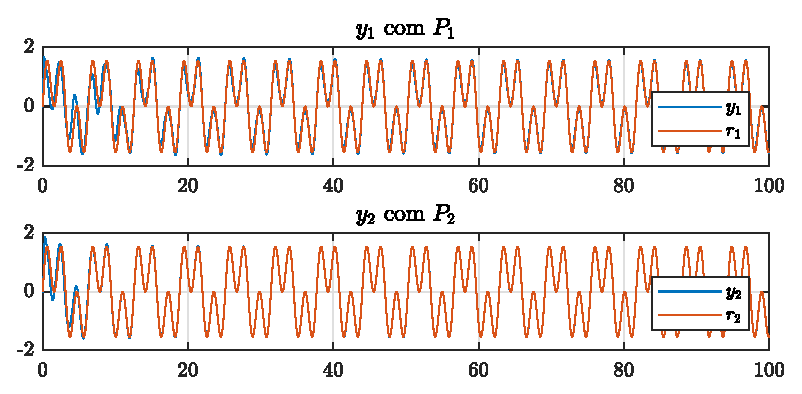
\includegraphics[width=12cm]{figs/y/P1P2.eps} 
\end{figure}

\begin{figure}[H]
  \centering
  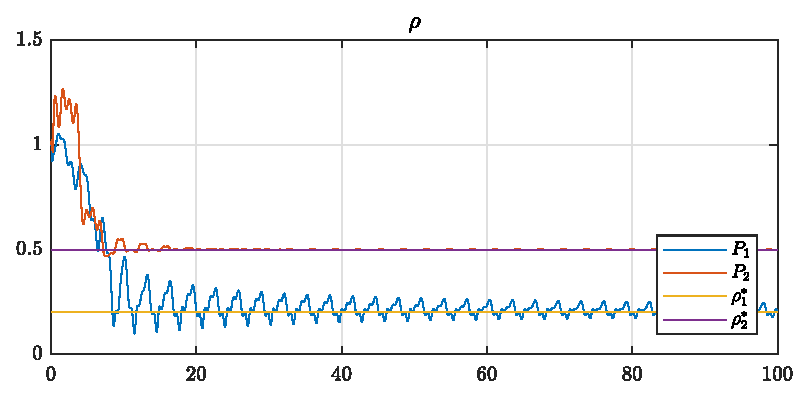
\includegraphics[width=12cm]{figs/rho/P1P2.eps} 
\end{figure}


\subsection{Simula��o \#3}

Verificamos o comportamento do sistema para varia��es no sinal de refer�ncia $y_r(t)$.

\begin{align*}
  y &= \frac{5}{s^2+2s+1}u\,,  & y(0) &=  0 \,, & \Gamma &= 1 \,
  \textbf{I}_3\,, & y_r &= \HI{$\textrm{sin}(t) + \textrm{sin}(3t)$} \,\, \textrm{e} \,\,
  \HI{$\textrm{sin}(t) + \textrm{2sin}(5t)$} \,.
\end{align*}

\begin{figure}[H] 
  \centering
  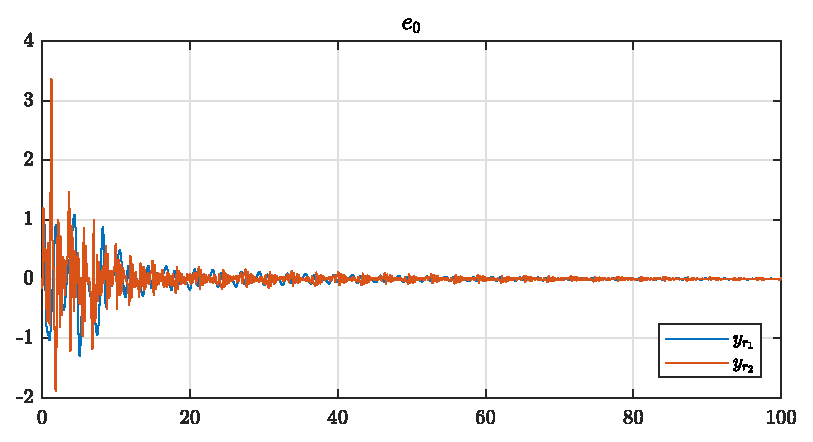
\includegraphics[width=12cm]{figs/e0/yr1yr2.eps} 
\end{figure}

\begin{figure}[H]
  \centering
  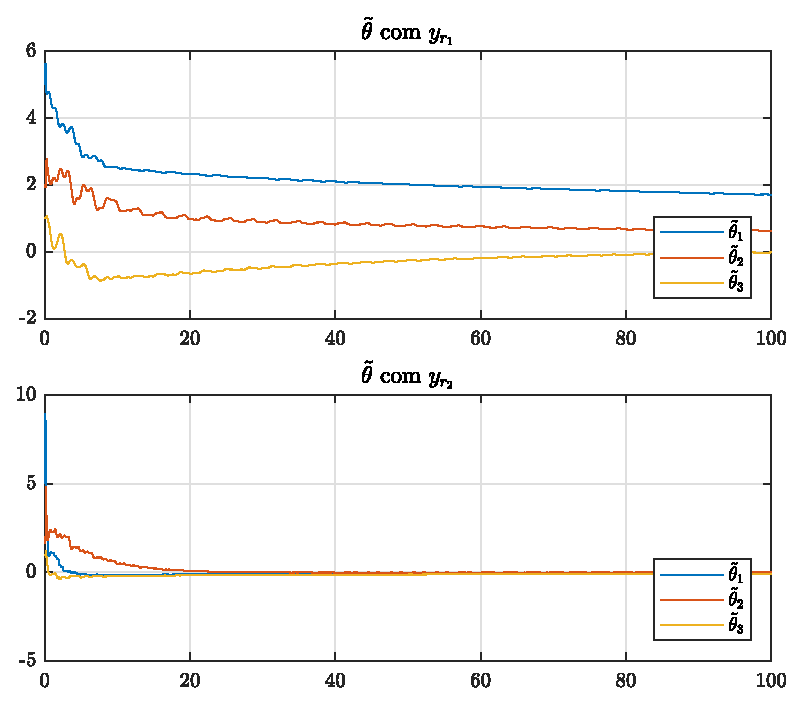
\includegraphics[width=12cm]{figs/tiltheta/yr1yr2.eps} 
\end{figure}

\begin{figure}[H]
  \centering
  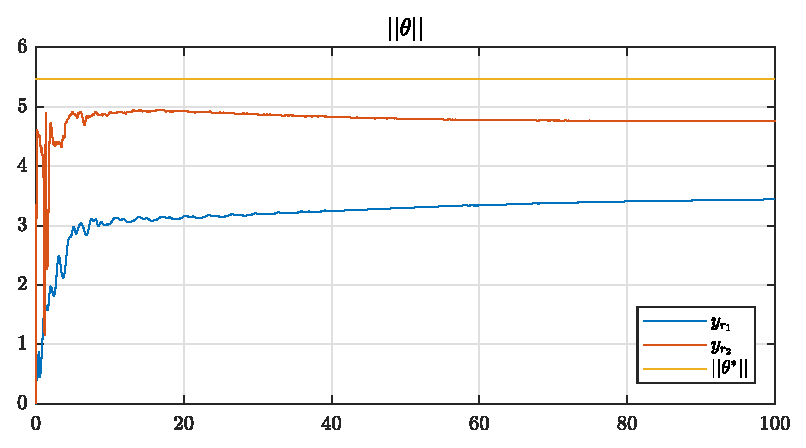
\includegraphics[width=12cm]{figs/modtheta/yr1yr2.eps} 
\end{figure}

\begin{figure}[H]
  \centering
  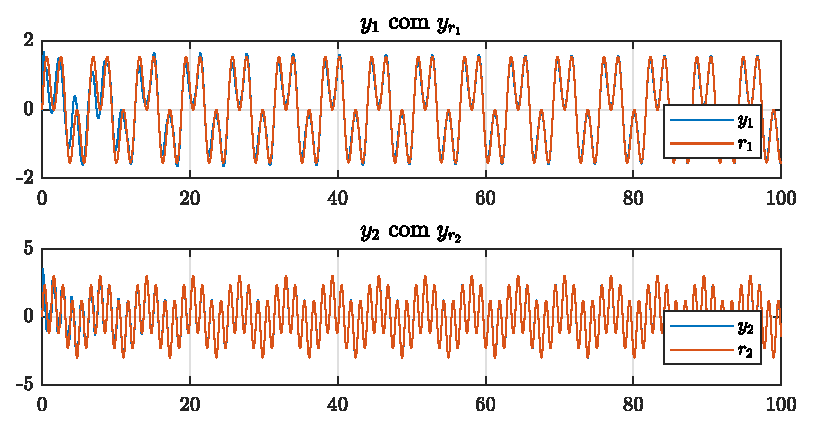
\includegraphics[width=12cm]{figs/y/yr1yr2.eps} 
\end{figure}

\begin{figure}[H]
  \centering
  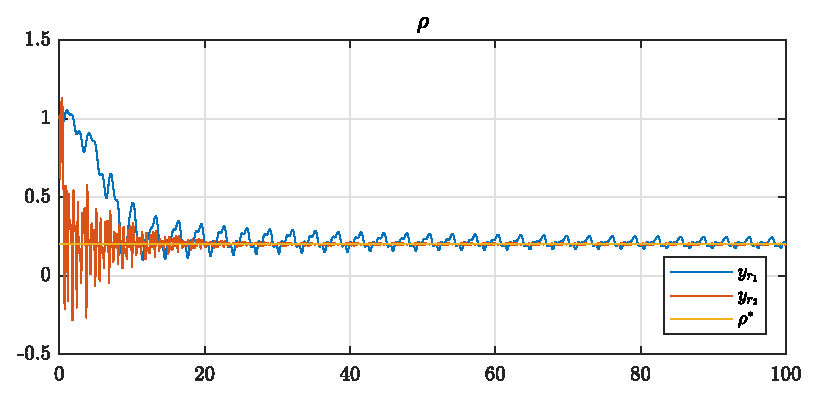
\includegraphics[width=12cm]{figs/rho/yr1yr2.eps} 
\end{figure}

\subsection{Simula��o \#4}

Verificamos o comportamento do sistema para varia��es no ganho de adapta��o $\Gamma$.

\begin{align*}
  y &= \frac{5}{s^2+2s+1}u\,,  & y(0) &=  0 \,, & \Gamma &= \HI{$1 \textbf{I}_3$} \,\, \textrm{e} \,\, \HI{$10 \textbf{I}_3$}\,, & y_r &= \textrm{sin}(t) + \textrm{sin}(3t) \,.
\end{align*}

\begin{figure}[H] 
  \centering
  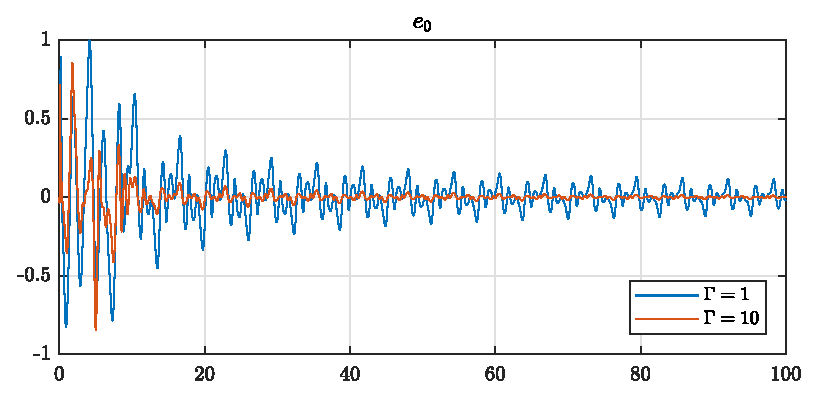
\includegraphics[width=12cm]{figs/e0/Gamma1Gamma10.eps} 
\end{figure}

\begin{figure}[H]
  \centering
  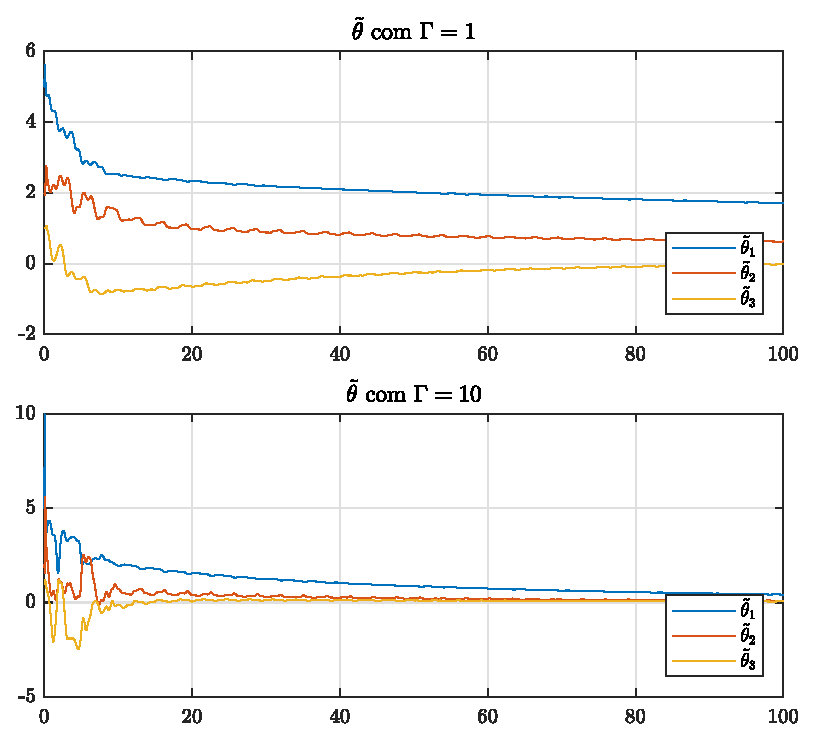
\includegraphics[width=12cm]{figs/tiltheta/Gamma1Gamma10.eps} 
\end{figure}

\begin{figure}[H]
  \centering
  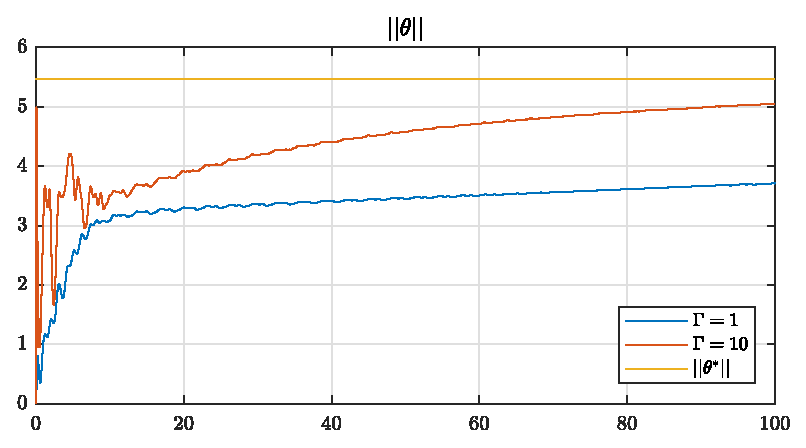
\includegraphics[width=12cm]{figs/modtheta/Gamma1Gamma10.eps} 
\end{figure}

\begin{figure}[H]
  \centering
  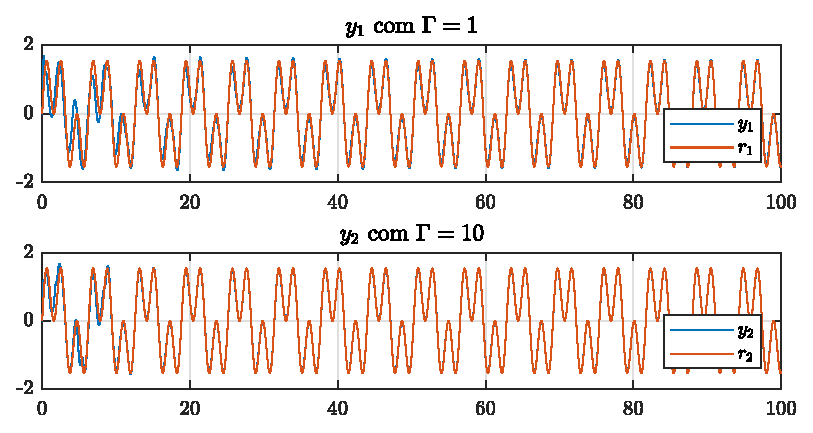
\includegraphics[width=12cm]{figs/y/Gamma1Gamma10.eps} 
\end{figure}

\begin{figure}[H]
  \centering
  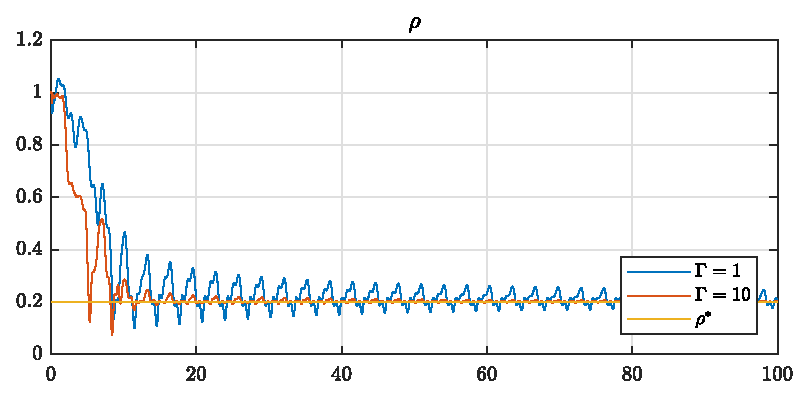
\includegraphics[width=12cm]{figs/rho/Gamma1Gamma10.eps} 
\end{figure}
